\section{Introduction}
\label{sec:intro}

We present \ourmodelfull, a Mixture-of-Experts (MoE) hybrid Mamba-Transformer model~\citep{lieber2024jambahybridtransformermambalanguage} with agentic, reasoning, and chat capabilities. Like previous generations~\citep{nvidia2025nemotronhfamilyaccurateefficient,nemotronnanov2}, \ourmodel uses a combination of Mamba-2~\citep{dao2024transformersssmsgeneralizedmodels} and Grouped-Query-Attention (GQA)~\citep{ainslie2023gqatraininggeneralizedmultiquery}. In addition, \ourmodel uses Mixture-of-Experts~\citep{shazeer2017outrageously} layers to scale model parameters sparsely and achieve significant improvements on the inference-throughput-to-accuracy frontier. We use a granular MoE architecture~\citep{dai2024deepseekmoe} with a learnt MLP router that activates 6 out of 128 experts~(\S\ref{sec:arch}). \ourmodel totals 31.6B parameters out of which only 3.2B are activated per forward pass (3.6B including embeddings). \ourmodel achieves better or on-par accuracy compared to GPT-OSS-20B~\citep{openai2025gptoss120bgptoss20bmodel} and Qwen3-30B-A3B-Thinking-2507~\citep{yang2025qwen3technicalreport} as shown in Figure~\ref{fig:intro}. Further, on the 8K input / 16K output token scenario,
\ourmodel provides 2.2$\times$ and 3.3$\times$ faster inference throughput compared to GPT-OSS-20B and Qwen3-30B-A3B-Thinking-2507 respectively. \ourmodel also supports context lengths up to 1M tokens, outperforming both GPT-OSS-20B and Qwen3-30B-A3B-Instruct-2507 on RULER across different context lengths. Along with the model weights, we provide the recipe, code, and most of the data we used to train the model.

\begin{figure}[ht]
    \centering
    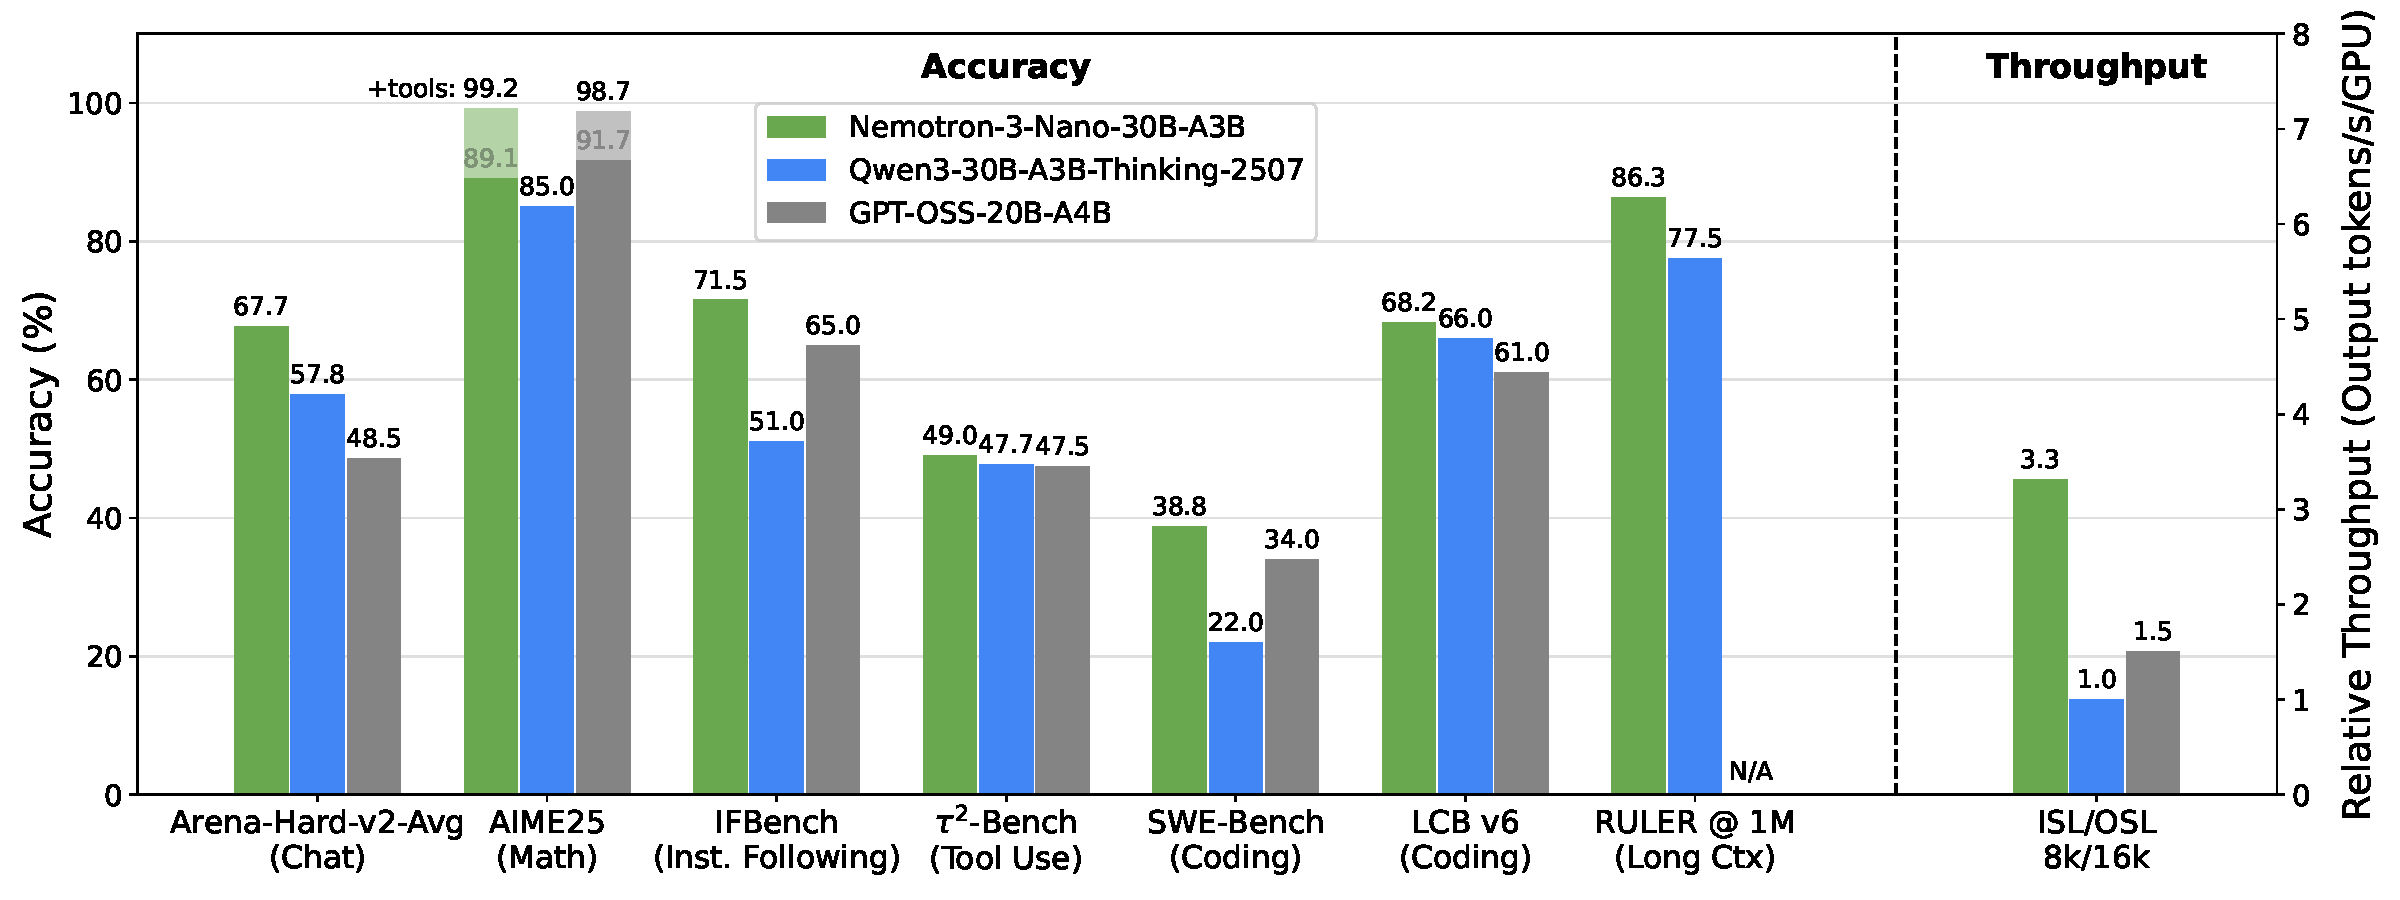
\includegraphics[width=\linewidth]{figures/nanov3_introfig.pdf}
    \caption{Accuracy and throughput comparisons of \ourmodel with Qwen3-30B-A3B-Thinking-2507 and GPT-OSS-20B. \ourmodel achieves on-par or better accuracies across multiple benchmarks. RULER scores for 1M context length are available only for \ourmodel and Qwen3 since GPT-OSS-20B has a context length of 128K tokens. Further, on 8K input / 16K output setting, \ourmodel provides inference throughput that is 3.3$\times$ higher than Qwen3-30B-A3B-Thinking-2507 and 2.2$\times$ higher than GPT-OSS-20B. We measured throughput on a single H200 GPU with vLLM and TRT-LLM and used the best out of the two for each model. We used the OpenHands harness to evaluate SWE-Bench.}%\todo{Roger: put with tool numbers in AIME25} \todo{Roger: write chat under arena-hard}} \todo{Roger: 48.3 in tau-Bench for nano-v3} \todo{Roger: Change Tau-Bench to $\tau^2$-Bench }
    \label{fig:intro}
\end{figure}


We pretrained our base model, \ourbasemodel, using the Warmup-Stable-Decay~\citep{hu2024minicpm} learning rate schedule on 25 trillion tokens of text data spanning 15 categories (\S\ref{sec:pretrain_data}). We divided pre-training into 2 phases with 23.5 trillion tokens of diverse data in the first phase, followed by 1.5 trillion tokens of high-quality data in the second phase (\S\ref{section:blend}). Our base model achieves better accuracy than equivalent-sized Qwen3-30B-A3B-Base on most academic benchmarks across Code, Math, Long Context, General Knowledge, and Commonsense Understanding categories. We do not compare the accuracy of our base model to GPT-OSS-20B because no base model was released with it.  Our model also achieves significantly better inference throughput than Qwen3-30B-A3B~(3.3$\times$) and GPT-OSS-20B~(2.2$\times$) on generation heavy 8K input / 16k output scenario when tested on a single H200 GPU. We measured throughput using the best configuration available for H200 GPUs with both vLLM and TRT-LLM and used the better of the two for each model. We used \texttt{FP8} for both weights and activations for throughput measurement of \ourmodel and Qwen3. We used \texttt{mxfp4} for weights and \texttt{bfloat16} for activations for GPT-OSS-20B.


We post-trained \ourmodel using three approaches: supervised fine tuning (SFT) (\S\ref{subsec:SFT}), multi-environment reinforcement learning from verifiable rewards (RLVR) (\S\ref{subsec:RLVR}), and reinforcement learning from human feedback (RLHF) (\S\ref{subsec:RLHF}). During SFT, we trained \ourmodel on a diverse set of chat, agentic, and reasoning traces to imbue the model with reasoning budget control, reasoning on/off control, and tool-integrated reasoning capabilities. During RLVR, we trained on all environments simultaneously, resulting in a smooth and uniform improvement in model capabilities. During RLHF, we utilized a large and accurate generative reward model (GenRM) to enhance the performance of \ourmodel on key chat benchmarks. %By scaling post-training in this manner, \ourmodel achieves best in class results across a wide variety of tasks.

We also quantized \ourmodel from \texttt{bfloat16} to \texttt{FP8} using post training quantization (PTQ). This helps achieve higher inference throughput with minimal loss in accuracy~(\S\ref{subsec:quantaccuracy}).

Along with this report, we are releasing the model recipes\footnote{\href{https://github.com/NVIDIA-NeMo/Nemotron}{https://github.com/NVIDIA-NeMo/Nemotron}} and publishing the following:

\newparagraph{Checkpoints}
\begin{itemize}
    % \item \href{}{\ourfinalmodel}: the final post-trained model
    % \item \href{}{\ourbasemodel}: the pre-trained base model
    \item \href{https://huggingface.co/nvidia/NVIDIA-Nemotron-3-Nano-30B-A3B-FP8}{\texttt{\ourfinalmodel FP8} 
\includegraphics[height=0.9em]{assets/huggingface-color.png}} : the final post-trained and FP8 quantized model 
    \item \href{https://huggingface.co/nvidia/NVIDIA-Nemotron-3-Nano-30B-A3B-BF16}{\texttt{\ourfinalmodel BF16} 
\includegraphics[height=0.9em]{assets/huggingface-color.png}} : the post-trained model
    \item \href{https://huggingface.co/nvidia/NVIDIA-Nemotron-3-Nano-30B-A3B-Base-BF16}{\texttt{\ourbasemodel BF16} 
\includegraphics[height=0.9em]{assets/huggingface-color.png}} : the pre-trained base model
    \item \href{https://huggingface.co/nvidia/Qwen3-Nemotron-235B-A22B-GenRM}{\texttt{\ourgenrm} 
\includegraphics[height=0.9em]{assets/huggingface-color.png}} : the GenRM used for RLHF
\end{itemize}

\newparagraph{Data}
\begin{itemize}
    \item \href{https://huggingface.co/datasets/nvidia/Nemotron-CC-v2.1}{\texttt{Nemotron-CC-v2.1} 
\includegraphics[height=0.9em]{assets/huggingface-color.png}} : 2.5 trillion new English tokens from Common Crawl, including curated data from 3 recent snapshots, synthetic rephrasing, and translation to English from other languages.
    \item \href{https://huggingface.co/datasets/nvidia/Nemotron-CC-Code-v1}{\texttt{Nemotron-CC-Code-v1} 
\includegraphics[height=0.9em]{assets/huggingface-color.png}} : A pretraining dataset consisting of 428 billion high-quality code tokens obtained from processing Common Crawl Code pages using the Lynx + LLM pipeline from \href{https://huggingface.co/datasets/nvidia/Nemotron-CC-Math-v1}{\texttt{Nemotron-CC-Math-v1} }. Preserves equations and code, standardizes math equations to LaTeX, and removes noise.
    \item \href{https://huggingface.co/datasets/nvidia/Nemotron-Pretraining-Code-v2}{\texttt{Nemotron-Pretraining-Code-v2} 
\includegraphics[height=0.9em]{assets/huggingface-color.png}} : Refresh of curated GitHub code references with multi-stage filtering, deduplication, and quality filters. Large-scale synthetic code data.
    \item \href{https://huggingface.co/datasets/nvidia/Nemotron-Pretraining-Specialized-v1}{\texttt{Nemotron-Pretraining-Specialized-v1} 
\includegraphics[height=0.9em]{assets/huggingface-color.png}} : Collection of synthetic datasets for specialized areas like STEM reasoning and scientific coding.
    \item \href{https://huggingface.co/collections/nvidia/nemotron-post-training-v3}{\texttt{Nemotron-SFT-Data} 
\includegraphics[height=0.9em]{assets/huggingface-color.png}} : Collection of new \ourmodel SFT datasets.
    \item \href{https://huggingface.co/collections/nvidia/nemo-gym}{\texttt{Nemotron-RL-Data} 
\includegraphics[height=0.9em]{assets/huggingface-color.png}} : Collection of new \ourmodel RL datasets.

\end{itemize}

% \newparagraph{Code}
% \begin{itemize}
%     \item \href{https://github.com/NVIDIA/Megatron-LM}{\texttt{https://github.com/NVIDIA-NeMo/Nemotron}}: Pretraining and SFT
% \end{itemize}
%Soumye : Confirm with Oleksii and others if we want to put Codebase links as highlight here too

% \newparagraph{Recipes}
% \begin{itemize}
%     \item \href{}{\texttt{Nemotron Recipes}}
% \end{itemize}

We divide the remainder of the report into 3 sections: Pre-training~(\S\ref{sec:pretraining}), Post-Training~(\S\ref{sec:alignment}), and Quantization~(\S\ref{sec:quantization}). 
